\section{Experiments} \label{experiments}

	\subsection{Experimental enviroments}
	
		Training a deep learning model that involves intensive compute tasks on large dataset can take days to run on a single CPU or a slow GPU. In our case, since HAM10000 dataset has 10015 images, it is unthinkable to perform the training of a convolutional neural network with a standard laptop. The solution turned to cloud computing. The choice fells on Google Cloud Platform because of the availability of free tier that consists in 300\$ free credits that can be used in any GCP product. 
		
		\smallskip
		
		We have tested our CNN models on a custom instance of Compute Engine. Our VM’s configuration is presented in Table \ref{tab:hw-config}
		
		\begin{table}[H]
			\centering
			\begin{tabular}{ |c|c|c|c|c|c| }
				\hline
				\textbf{Operating System} & \textbf{CPU} & \textbf{Memory} & \textbf{Disk} & \textbf{GPU} \\ \hline
				
				Ubuntu 18.04 LTS & 8 core & 52 GB & SSD / 100 GB & 1x NVIDIA Tesla K80 \\ \hline
				
			\end{tabular}
			\caption{Virtual machine configuration}
			\label{tab:hw-config}
		\end{table}
	
		Our models have been implemented in keras using tensorflow as a backend. The code is available on our GitHub repository: \url{https://github.com/albertobezzon/cognitiveservices}
		
	\subsubsection{Proposed model performances}
	
		In Figure \ref{fig:first-matrix} we show the performances of our proposed model on the test set. It is possible to see that our model has difficulties in predicting Dermatofibromas (only 11\% correctly classified) and Melanomas (only 27\% correctly classified).In particular, Dermatofibromas are confused with basal cell carcinomas (33\% of Dermatofibromas are classified like a basal cell carcinoma) and Melanocytic Nevis (33\% of Dermatofibromas are classified like a Melanocytic nevi), while Melanomas are confused with Melanocytic nevis (46\% of Melanomas are classified like a nevi). 
		This means that these classes are similar in terms of features and the imbalanced of the dataset doesn’t help in discriminating well between them. We have too few examples for Dermatofibromas and too much examples for Melanocytic Nevis. Similar problems are also present in few of the other classes.
		
		\begin{figure}[H]
			\centering
			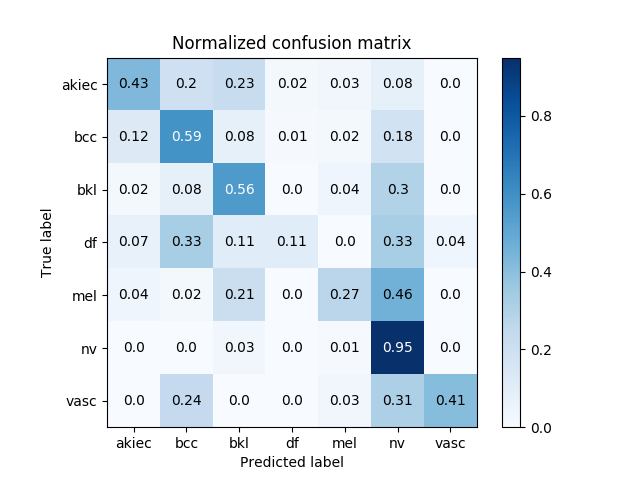
\includegraphics[width=15cm]{images/firstMatrix.png}
			\caption{Confusion matrix}
			\label{fig:first-matrix}
		\end{figure}
		
	\subsubsection{Class weighting}
	
		The first technique we tried to deal with the problem of imbalanced data is class weighting. This technique consists in assigning a weight to each class in such a way that allows to the model to give more emphasis to minority classes and less emphasis to majority classes. The idea is to assign more priority to the classes with less examples and less priority to the classes with more examples. In this way it is possible to balance the training set for the model. 
		In Figure \ref{fig:second-matrix} we show the performances of our proposed model on the test set with the class weighting technique.
		Even if the test accuracy of the model with class weighting is lower (65\% against 77\% of the previous model), it is possible to see that the correct classifications are better distributed over all the classes and this is our main goal. In fact, with class weighting the 48\% of Dermatofibromas is correctly classified and the 53\% of Melanomas. Moreover, it seems that with the class weighting our proposed model is able to distinguish better between Dermatofibromas and Melanocytic nevis, but also between Melanomas and Melanocytic nevis. Finally, it seems that also the number of misclassified examples is better distributed on the matrix. There are still difficulties in distinguishing between Dermatofibromas and Basal cell carcinoma, but we think it is possible to make the model more accurate with more training data.
		
		\begin{figure}[H]
			\centering
			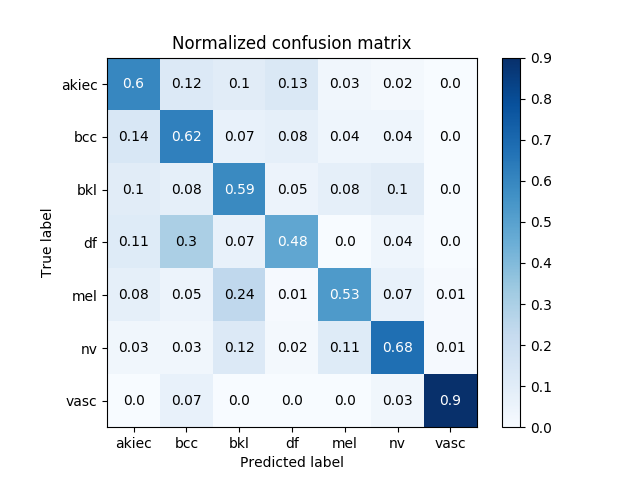
\includegraphics[width=15cm]{images/secondMatrix.png}
			\caption{Confusion matrix}
			\label{fig:second-matrix}
		\end{figure}
		
	\subsubsection{Oversampling with data augmentation}
	
		The last experiment we tried on HAM10000 is the oversampling of minority classes with data augmentation. After splitting the dataset as reported in Section \ref{dataset}, the number of examples in Melanocytic nevis class was 4868, so we applied data augmentation to all the other classes to obtain a balanced training set. After applying these procedures, we obtained a 34.076 images training set.
		To oversampling the training set we have used keras' ImageDataGenerator with the following parameters:
		\begin{itemize}
			\item rotation range: 45; 
			\item zoom range: 0.2; 
			\item width shift range: 0.1;
			\item height shift range: 0.1;
			\item horizontal flip: true; 
			\item vertical flip: true;
			\item fill mode: nearest.
		\end{itemize}
		
		After data augmentation we checked that the generated images were good and then we trained our proposed model on the augmented training set.
		In Figure \ref{fig:third-matrix} we show the performances on the test set of our proposed model with the oversampling technique.
		
		\begin{figure}[H]
			\centering
			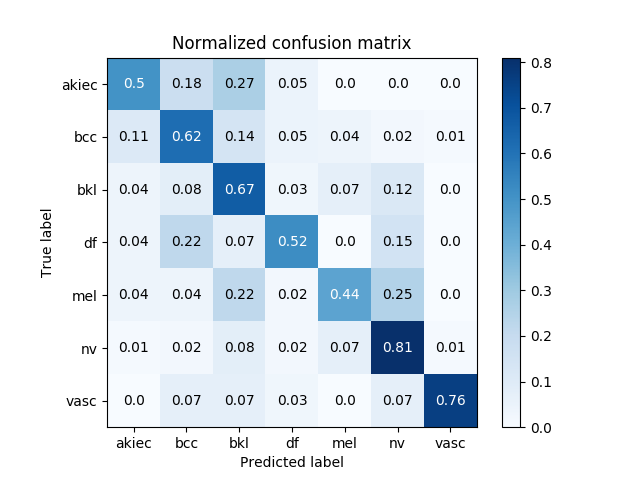
\includegraphics[width=15cm]{images/thirdMatrix.png}
			\caption{Confusion matrix}
			\label{fig:third-matrix}
		\end{figure}
		
		Unfortunately, we did not achieve the desired results, in fact even if the model trained on oversampled dataset is better in predicting Dermatofibromas (52\% well classified Dermatofibromas against 48\% of the previous model), and this explains the higher macro average F1 (0.56 against 0.51), it reintroduces difficulties in distinguish between Melanomas and Melanocytic nevis (25\% of Melanomas are classified like a Melanocytic nevi). 
		Moreover, due to aggressive data augmentation (we added more than 4000 augmented images to Dermatofibroma class) the model tends to badly overfit, even if regularizations techniques are configured. In Figure \ref{fig:overfitting-data-aug} is possible to see the overfitting of this last model.
		
		\begin{figure}[H]
			\centering
			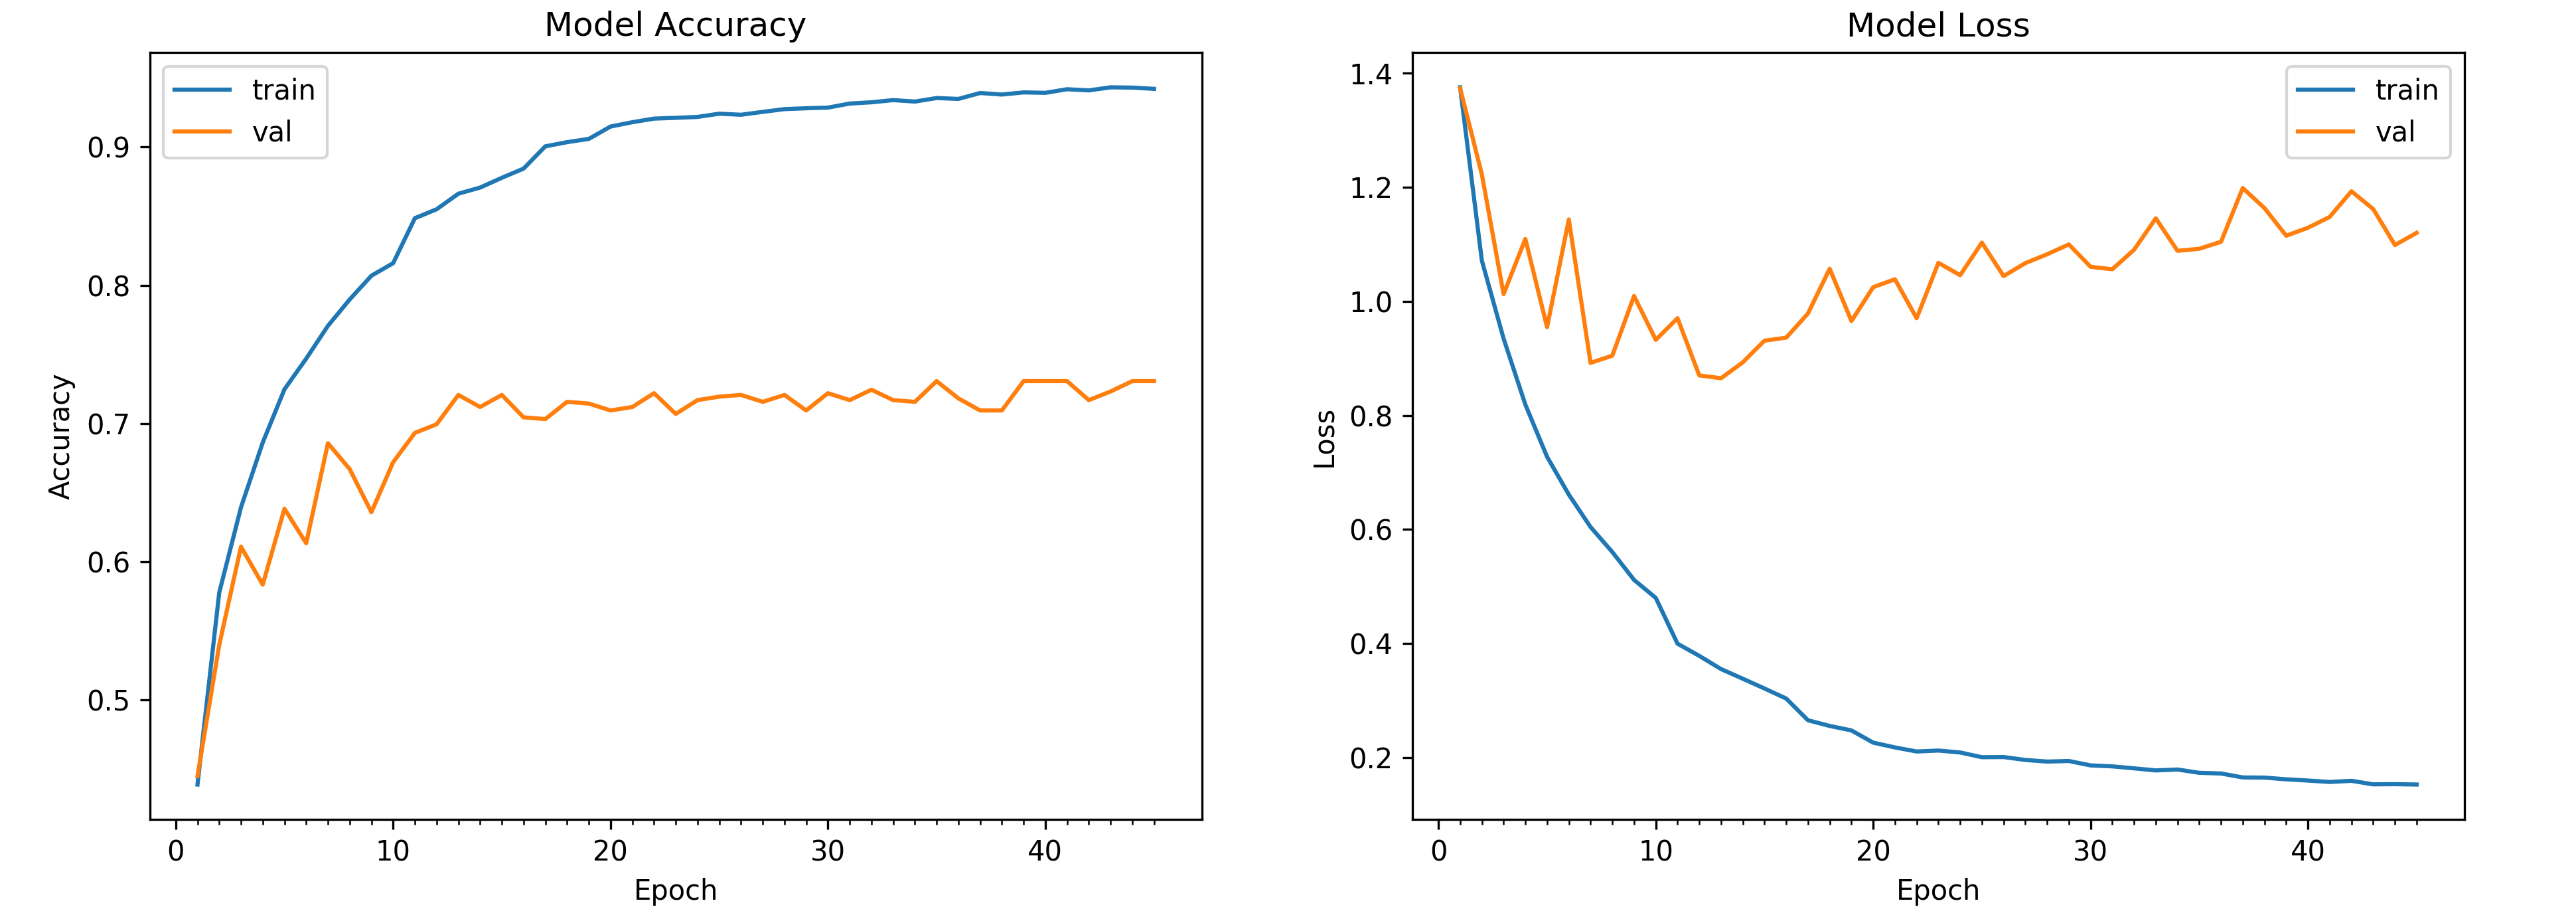
\includegraphics[width=15cm]{images/overfitting-data-aug.png}
			\caption{Plot of accuracy and loss of data augmented model}
			\label{fig:overfitting-data-aug}
		\end{figure}
		
		In Table \ref{tab:experiments_results} is possible to compare the performances on the test set of the previous three models in terms of F1 scores, macro average F1 and accuracy.
		
		\begin{table}[H]
			\centering
			\begin{tabular}{ |>{\centering\arraybackslash}p{2.5cm}|c|c|c|c|c|c|c|>{\centering\arraybackslash}p{1.5cm}|>{\centering\arraybackslash}p{2cm}| }
				\hline
				\textbf{Model} & \textbf{akiec} & \textbf{bcc} & \textbf{bkl} & \textbf{df} & \textbf{mel} & \textbf{nv} & \textbf{vasc} & \textbf{Macro average} & \textbf{Test accuracy} \\ \hline
				
				Proposed model & 0.44 & 0.55 & 0.54 & 0.17 & 0.39 & 0.90 & 0.56 & 0.51 & 0.77 \\ \hline
				Class weighting & 0.38 & 0.50 & 0.45 & 0.27 & 0.48 & 0.80 & 0.71 & 0.51 & 0.65 \\ \hline
				Oversampling & 0.46 & 0.54 & 0.53 & 0.34 & 0.47 & 0.86 & 0.75 & 0.56 & 0.72 \\ \hline
				
			\end{tabular}		
			\caption{Experiments' results}
			\label{tab:experiments_results}
		\end{table}
	
		The model trained on the oversampled training set gives better results in terms of performance measures compared to the other models, but tends to misclassify too much Melanomas, that are the most important class for our goal.
		So, in conclusion, even if the last model performs relatively well, we prefer to select the model with class weighting as our best model because it has performances that better meet our goal of reducing the number of misclassified skin lesions.
		
		
		
		
		